\chapter{System Design}

%%======================================================================%%
\section{Preprocessing}

\subsection{Resampling}
An unfortunate disadvantage of the Android platform is that Android does not guarantee an even sampling rate on its sensors. In lieu of defining a sampling rate, Android allows the developer to request the delay amount between sensor readings. These delays can be \textit{NORMAL, GAME, UI,} or \textit{FASTEST}, going from a $200000\mu s$ delay down to a zero second delay.

Likewise, although Android does not allow us to define a sampling rate, setting the delay to \textit{FASTEST} results in a sampling rate consistently near 25Hz. To be precise, the accelerometer was measured to have a sampling rate of approximately 24.67Hz on average. This is however an average, thus samples may come early or late, depending on how the Android scheduler prioritizes sensor readings. 

Because of this, we resample with a zero-order hold (ZOH). ZOH is very easy to implement, and considering how close our sampling rate is to our desired rate of 25Hz, we maintain a high fidelity signal. Any additional noise introduced due to resampling is effectively filtered out in our next step.

\subsection{Filtering}
Repetitions occur generally on the order of 1Hz, and bodybuilding exercises tend not to have many sharp movements due to the threat of injury, thus we decide on a frequency cutoff of 12Hz for our signal. This is conveniently in the middle of our (now resampled) sampling rate, and it will take care of noise added in the previous step.

Our low-pass filter is implemented using a unity-gain five-tap IIR Butterworth filter generated in MATLAB.


%%======================================================================%%
\section{Segmentation}

Sensor data is sent in batches from the watch to reduce message overhead and preserve battery life, thus segmentation must be able to handle large amounts of data at each iteration.

\begin{figure}
    \centering
    \resizebox{\textwidth}{!}{
        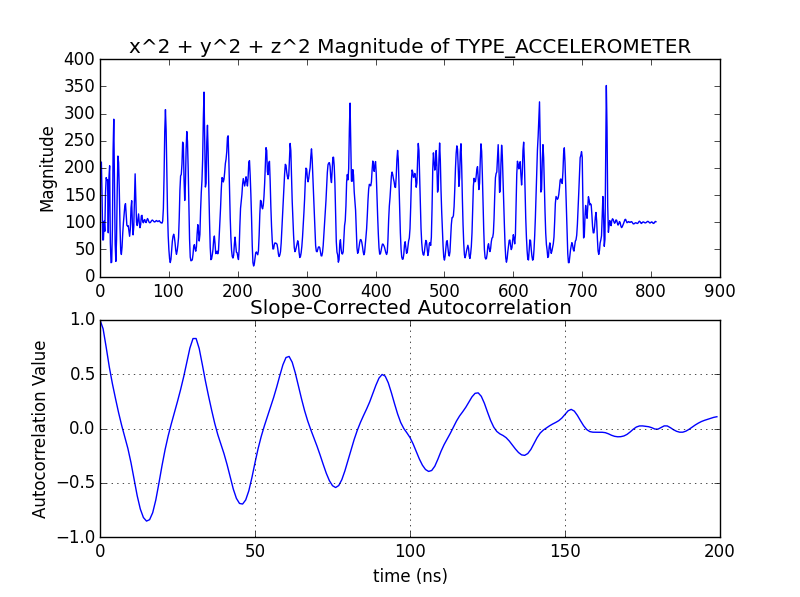
\includegraphics{curl_magnitude_autoc}
    }
    \caption{Autocorrelation of a periodic signal}
\end{figure}

\begin{figure}
    \centering
    \resizebox{\textwidth}{!}{
        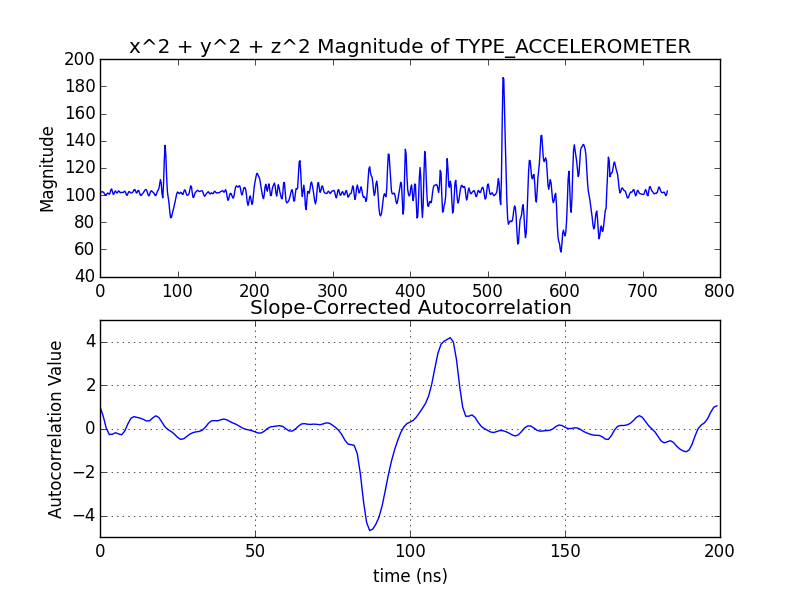
\includegraphics{noisy_no_exercise_autoc}
    }
    \caption{Autocorrelation of an aperiodic signal}
\end{figure}

\subsection{Sliding Window Buffers}
First, our data is split into 5s buffers using a sliding window with 4.8s overlap. This is done for the purposes of autocorrelation. As mentioned earlier, we expect exercise to be roughly periodic across the entire signal, exhibiting an autocorrelation similar to Figure 4.1, contrasted to aperiodic movement as in Figure 4.2. This is not entirely the case, however. Anecdotally, when performing a set of ten repetitions, the first repetitions will be done better than the final repetitions. Bar speed is directly indicative of the quality of a repetition, thus early repetitions are performed quicker than later repetitions. Computing autocorrelation over the entire signal would not make sense then - concurrent repetitions will likely be similar, but the first is nearly guaranteed to have a different period than the last. Therefore, we compute segmentation over sliding windows. 

\subsection{Signal Variants}
Our system uses two three-axis sensor sources: the smartwatch's accelerometer and gyroscope. We derive the following signals from each sensor stream:

\begin{enumerate}
    \item \textbf{X-axis:} the X-axis of the accelerometer/gyroscope
    \item \textbf{Y-axis:} the Y-axis of the accelerometer/gyroscope
    \item \textbf{Z-axis:} the Z-axis of the accelerometer/gyroscope
    \item \textbf{Magnitude:} the $\sqrt{x^2 + y^2 + z^2}$ magnitude of the accelerometer/gyroscope
    \item \textbf{PCA:} the projection of the three-axis data onto its first principal component
\end{enumerate}

This results in 10 total signals, 5 for each sensor. In the past, the orientation of the IMU could not be determined a priori, thus only the axis pointing along the direction of the arm could be used. We can make stronger assumptions however with the use of Android Wear, as a smartwatch has only one possible orientation on the wrist. This allows us to use all three axes as raw signals.

Included in this set are two derived signals, magnitude and PCA. Both signals are attempts at illustrating the primary axis of movement, with magnitude being a crude estimate and the projection onto the raw signal's first principal component being a more refined estimate. In our trials, we have found that computing both the primary projection and the magnitude signals is computationally inexpensive, thus both are used. Further investigation is required to determine if using both is necessary for sufficient classification, although the gain in omitting one is minimal.

\subsection{Feature Selection} 
From each of the ten sensor streams, we compute 29 features: 

\begin{enumerate}
    \item \textbf{Autocorrelation Features:}
    \begin{enumerate}
        \item \textbf{Total Number of Autocorrelation Peaks:} After computing autocorrelation, the total number of local maxima across the signal is recorded. For exercise, we expect this number to be on the order of two to five. An autocorrelation with no peaks implies idling, and an autocorrelation with too many peaks implies random movement.
        \item \textbf{Number of Prominent Autocorrelation Peaks:} Prominent peaks are determined using a threshold heuristic. If they are relatively isolated from surrounding peaks, and they are also greater in magnitude than surrounding peaks, they are considered prominent. We expect this to be close to the total number of autocorrelation peaks for exercise.
        \item \textbf{Number of Weak Autocorrelation Peaks:} Likewise, weak peaks are determined using the inverse of the strategy above. This should be close to the total number of peaks during non-exercise.
        \item \textbf{Maximum Autocorrelation Peak Value:} A large autocorrelation peak value implies high similarity between the original signal and the delayed version of the signal, indicating periodicity.
        \item \textbf{First Autocorrelation Peak Value:} Likewise, we expect the first peak to be very large for exercise. There is no such expectation for non-exercise.
        \item \textbf{First and Maximum Peak Values Equal:} Finally, the first peak is what we use to determine the period of the signal during exercise. If this first peak is also the largest in the autocorrelated signal, we are likely to be exercising.
    \end{enumerate}        
    \item \textbf{Energy Features:}
    \begin{enumerate}
        \item \textbf{RMS Amplitude:} RMS amplitude is computed for the full window, the first half of the window, and the second half of the window to account for when the window lies on an exercise boundary. Additionally, the CUSUM RMS amplitude is computed as a loose approximation of velocity RMS amplitude.
        \item \textbf{Power Spectrum Bin Magnitudes:} The power spectrum is binned into 10 equally wide segments and recorded. 
    \end{enumerate}
    \item \textbf{Statistical Features:} Similar to RMS, the following features are computed for the full window, the first half of the window, and the second half of the window: 
    \begin{enumerate}
        \item \textbf{Mean} 
        \item \textbf{Variance}
        \item \textbf{Standard Deviation}
    \end{enumerate}
\end{enumerate}

This results in a total of 291 features, which are passed into a classifier. 

\subsection{Classification}
These features are passed into a binary SVM trained using athletes familiar with each lift. We then use an accumulator-style voting system to determine when an exercise boundary has been crossed. If the SVM predicts that a lift is occurring, we increment the accumulator. Likewise, if it predicts non-exercise, we decrement the accumulator. Once an accumulator threshold is crossed, we can say with relative certainty that exercise is occurring. The same is done in reverse for computing the end of an exercise boundary.

In practice, we set an accumulator threshold equal to two seconds of activity. Two seconds tends to be the time it takes to complete one full repetition and begin another repetition. This could be increased to reduce false positives, although computing an accurate exercise window boundary is important for counting the number of repetitions. This becomes more difficult as the accumulator threshold increases.

%%======================================================================%%
\section{Recognition}

The recognition phase follows a similar structure as the segmentation phase. From the segmentation phase, we receive a set of data indices bounding the beginning and end of an exercise window. This window is then broken down into five second buffers with 4.8s overlap. The same set of five signals per sensor source is also calculated, those being the \textbf{X, Y, and Z axes, the signal magnitude, and the signal's primary PCA projection}. The main difference however is in the features extracted.

\subsection{Feature Selection}
Autocorrelation is useful for estimating whether a signal is periodic as well what its period may be, but we cannot use that information for recognition. Training a classifier which depends on bar speed would be inherently erroneous, as bar speed varies wildly depending on strength, stamina, and lift intensity. To this end, we omit most autocorrelation features from the segmentation phase and focus on other features:

\begin{enumerate}
    \item \textbf{Autocorrelation Features:}
    \begin{enumerate}
        \item \textbf{Autocorrelation Bins:} Compute the autocorrelation of the window and instead of searching for peaks, compute the magnitude for 10 evenly-spaced bins.
    \end{enumerate}
    \item \textbf{Energy Features:}
    \begin{enumerate}
        \item \textbf{RMS:} The RMS of the full window is computed. 
        \item \textbf{Power Spectrum Bin Magnitudes:} Similar to the segmentation phase, the power spectrum is split into 10 evenly-spaced bins, and the magnitudes of each are recorded.
    \end{enumerate}
    \item \textbf{Statistical Features:}
    \begin{enumerate}
        \item \textbf{Mean}
        \item \textbf{Standard Deviation}
        \item \textbf{Kurtosis}
        \item \textbf{Interquartile Range}
    \end{enumerate}
\end{enumerate}

This results in a total of 200 features, which are passed into a classifier.

\subsection{Classification}
Classification is performed using a multi-class SVM. Predictions are made for each sliding window across the full exercise buffer and aggregated, with a final majority voting system determining which lift was performed during this segment.

%%======================================================================%%
\section{Counting}

The counting phase is performed over the primary PCA projection of the accelerometer, as this axis contains the majority of the signal's energy by definition. The accelerometer signal is chosen over the gyroscope signal as bar acceleration necessarily changes at the top and bottom of each lift, whereas rotation should not change at the top and bottom when performed correctly for most lifts.

Our counting algorithm can be defined by the following algorithm: 
\begin{enumerate}
    \item 
    \begin{enumerate}
        \item Find all local maxima in the signal
        \item Sort by amplitude
        \item For each peak, add the index to a set of candidate peaks if the distance to any other peak already in the set is at least MIN\_PERIOD away
    \end{enumerate}
    \item For each candidate peak:
    \begin{enumerate}
        \item Compute autocorrelation in a 5s window about the peak
        \item Find the maximum value in the autocorrelation, determining local periodicity P
        \item Remove peak from candidate set if it is $<0.75P$ away from any other peak
    \end{enumerate}
    \item 
    \begin{enumerate}
        \item Find the peak at the 40th percentile
        \item Reject any peaks smaller than half the amplitude of the 40th percentile peak
        \item Return the total number of remaining peaks as our final count
    \end{enumerate}
\end{enumerate}

MIN\_PERIOD is defined as the minimum amount of time a particular lift has ever taken to complete. This number is typically around 0.5s. 

Figures 3.2 and 3.3 illustrate the difficulties with counting. For an isolation exercise such as a bicep curl, repetitions tend to be clean, and peaks can be easily counted. Contrast this with a compound movement such as a bench press or a squat; it can be difficult to discern repetitions even when manually examining the signal.

\subsection{Algorithm Part 1}
Our first step in counting repetitions is to compile an initial list of peaks. We make an assumption that two repetitions could never occur within MIN\_PERIOD of each other, and so if two peaks are ever within that range, we assume they correspond to the same repetition. A prime example of this occurring is on Pendlay row; if the repetition is explosive enough, the bar will first accelerate off the floor, then it will experience another spike when it collides with the user's chest. 

\subsection{Algorithm Part 2}
Next, we further cull the candidate peak set by iterating through the list and determining the local period about each peak. If any surrounding peaks are too close, we remove them from the list. This segment works on the principle of self-similarity between concurrent repetitions. 

Speaking generally, Part 2 is a more liberal implementation of Part 1. In Part 1, we assume that the user could be lifting extremely quickly and allow for peaks that indicate rapid repetitions. In Part 2, we relax this assumption and compute what rate the user is actually lifting at, removing peaks that are notably faster. 

\subsection{Algorithm Part 3}
At this point, we have a well-formed candidate peak set, although there could still be peaks remaining that correspond to noise. For example, if a user stops at the top of a squat to catch his or her breath, there could be a peak when they readjust their position. This would not be removed using the autocorrelation method, thus it would be prudent to make one final pass through our candidate peak list to remove small peaks. 

Sorting our list by peak value, a seemingly accurate threshold would be at half the 40th percentile peak value. Few true peaks are less than that, so we can safely remove them. 

The size of the candidate peak set is then returned as our total number of repetitions.